\documentclass[border=30pt]{standalone}
\usepackage{amsmath}
\usepackage{xcolor}
\usepackage{tikz}
\usetikzlibrary{shadows}

\pagecolor{yellow!10}

\begin{document}
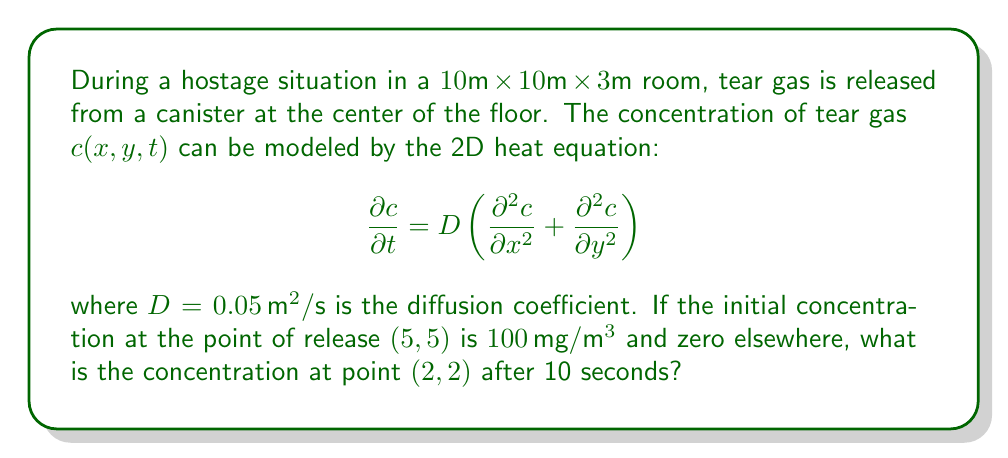
\begin{tikzpicture}
\node[draw=green!40!black, fill=white, line width=1pt, rounded corners=10pt, 
      text=green!40!black, font=\normalsize\sffamily, 
      text width=11cm, align=left, 
      drop shadow={shadow xshift=5pt, shadow yshift=-5pt, fill=gray!70},
      inner sep=15pt] 
{
During a hostage situation in a $10\text{m} \times 10\text{m} \times 3\text{m}$ room, tear gas is released from a canister at the center of the floor. The concentration of tear gas $c(x,y,t)$ can be modeled by the 2D heat equation:
\[
\frac{\partial c}{\partial t} = D \left( \frac{\partial^2 c}{\partial x^2} + \frac{\partial^2 c}{\partial y^2} \right)
\]
where $D = 0.05\,\text{m}^2/\text{s}$ is the diffusion coefficient. If the initial concentration at the point of release $(5,5)$ is $100\,\text{mg}/\text{m}^3$ and zero elsewhere, what is the concentration at point $(2,2)$ after 10 seconds?
};
\end{tikzpicture}
\end{document}
